\question 在可靠传输机制中,发送窗口的位置由窗口前沿和后沿的位置共同确定,经过一段时间,发送窗口的后沿的变化情况可能为(
)。 Ⅰ.原地不动 Ⅱ.向前移动 Ⅲ.向后移动
\par\twoch{Ⅰ、Ⅲ}{\textcolor{red}{Ⅰ、Ⅱ}}{Ⅱ、Ⅲ}{都有可能}
\begin{solution}发送窗口的后沿的变化情况只能有两种: 1)原地不动(没有收到新的确认)。
2)向前移动(收到了新的确认)。
发送窗口不可能向后移动,因为不可能撤销已收到的确认。
\end{solution}
\question 在滑动窗口流量控制中,若窗口大小为7,则ack=5意味着接收方期待的下一帧是(
)号帧
\par\twoch{7}{6}{\textcolor{red}{5}}{4}
\begin{solution}ack=n表示到n-1帧为止的所有帧都已经收到,接收方期待的下一帧为编号为n的帧。因此,ack=5表示接收方期待的下一帧是5号帧。
\end{solution}
\question 采用滑动窗口机制对发送方和接收方的通信过程进行流量控制。假定帧的序号长度是3,发送窗口和接收窗口的大小都是7。当A发送了编号0、1、2、3、4这5个帧后,B也接受了这5个帧,但仅应答了0、1两个帧,此时发送窗口将要发送的帧序号和接收窗口的上边界对应的帧序号是
\par\twoch{5,0}{\textcolor{red}{5,5}}{2,0}{2,3}
\begin{solution}发送窗口的大小决定了发送方在收到第一个确认帧之前可以发送的帧的数量,现在发送方窗口大小为7,说明发送方在收到第一个确认帧前可以发送7个帧,现在已经发送了5个帧(下一个应该发送5号帧),并收到了两个确认帧,故还可以发送7-5+2=4个帧,而接收方只要接收到一个帧上边界就会右移,跟是否返回确认帧无关,其实从上面的分析可以看出,返回的确认影响的是发送方,现在接收方接收了0、1、2、3、4这5个帧,要接收的帧序列是5、6、7、0、1、2、3,即上边界为5。
注:一般不予以说明,窗口的上边界是下一个期望序列号expectedSeq;下边界是起始序列号startSeq。
\end{solution}
\question 若数据链路的发送窗口大小为6,现在正在发送4号帧,当发送方接到3号帧的确认帧后,发送方还可连续发送的帧数是
\par\twoch{2}{3}{4}{\textcolor{red}{5}}
\begin{solution}发送方接收到3号帧的确认,说明到3号帧为止的所有帧都接收了,分析知发送方只有4号帧还未收到确认帧,而窗口大小为6,故发送方还可继续发送5个帧。
\end{solution}
\question 下列哪一项最能描述窗口的大小?
\par\fourch{软件允许并能迅速处理数据的窗口的最大值}{\textcolor{red}{等待一个确认时能传送的信息量}}{为使数据能发送,必须提前建立的窗口大小}{监视程序打开的窗口大小,它并不等于监视程序的大小}
\begin{solution}窗口大小是``等待一个确认时能传送的信息量''。
\end{solution}
\question 若采用后退N帧ARQ协议进行流量控制,帧编号字段为7位,则发送窗口的最大长度为
\par\twoch{7}{8}{\textcolor{red}{127}}{128}
\begin{solution}为了使接收方可以区分发送的帧是新帧还是重发的旧帧,在后退N帧ARQ协议中规定:若帧编号为n位,则发送窗口的大小Ws≤
\includegraphics[width=0.46875in,height=0.13542in]{texmath/9438eb5Cdpi7B3507D25En-1}。故当n=7时,发送窗Ws≤127
\end{solution}
\question 使用后退N帧协议,根据图3-17所示的滑动窗口状态(发送窗口大小为2,接收窗口大小为1),指出通信双方处于何种状态( )。(提示:发送方阴影部分表示已经发送的帧,但是没有收到确认;接收方阴影部分表示期待接收的帧。)
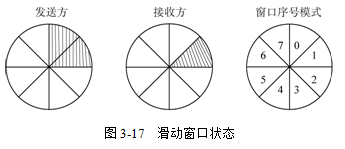
\includegraphics[width=3.33333in,height=1.43750in]{computerassets/36D7EBAA3994386EFBA3FD7C902040C5.png}
\par\fourch{发送方发送完0号帧,接收方准备接收0号帧}{\textcolor{red}{发送方发送完1号帧,接收方接收完0号帧}}{发送方发送完0号帧,接收方准备接收1号帧}{发送方发送完1号帧,接收方接收完1号帧}
\begin{solution}滑动窗口的本质是在任何时刻,发送方总是维持着一组序列号,分别对应于允许发送的帧,称这些帧落在发送窗口之内。发送窗口内的序列号代表了那些已经被发送,但是还没有被确认的帧。类似地,接收方也维持着一个接收窗口,对应于一组允许它接收的帧。从图3-17中可以看出,发送方已经发送了0号帧和1号帧,而接收方已经接收完了0号帧,并且对0号帧发回了确认,才使得接收窗口后移到1号帧位置。
\end{solution}
\question 数据链路层采用选择重传协议(SR)传输数据,发送方已发送了0\textasciitilde{}3号数据帧,现已收到1号帧的确认,而0,2号帧依次超时,则此时需要重传的帧数是(
)
\par\twoch{1}{\textcolor{red}{2}}{3}{4}
\begin{solution}知识点复习:
如果采用选择重传协议,若一帧出错,其后续帧先存入接收方的缓冲区中,同时要求发送方重传出错帧,一旦收到重传帧后,就和原先存在缓冲区的其余帧一起按正确的顺序送主机。所以,选择重传协议是不支持累积确认的,这一点需要和后退N帧协议区分开。
由于发送方只收到1号帧的确认,0,2号帧超时,由于不支持累积确认,所以需要重传0,2号帧。为什么不选择C?难道3号帧不需要重传吗?不需要,因为题干已经很清楚地说明了``此时``二字,此时也就是2号帧超时的时间,所以无需考虑3号帧的状态。
如果此题改为数据链路层采用后退N帧协议(GBN)传输数据,由于后退N帧协议具有累积确认的作用,故只需重传2号帧以及后续所有的帧,答案仍然选B。
【总结】
若采用n个比特对帧进行编号,选择重传协议的发送窗口尺寸WT必须满足:1
\end{solution}
\question 主机甲与主机乙之间使用后退N帧协议(GBN)传输数据,甲的发送窗口尺寸为1000,数据帧长为1000字节,信道带宽为100Mbps,乙每收到一个数据帧立即利用一个短帧(忽略其传输延迟)进行确认。若甲乙之间的单向传播时延是50
ns,则甲可以达到的最大平均数据传输速率约为( )
\par\twoch{10Mbps}{20Mbps}{\textcolor{red}{80Mbps}}{100Mbps}
\begin{solution}本题考察的是最大传输速率的计算,同时结合了滑动窗口协议中GBN协议的考察,题目问的是最大平均数据传输速率,那么我们就应当从如何达到最大这个临界点出发去考虑,根据GBN的规则,发送方可以连续发送数据帧,接收方每接收到一个数据帧之后都要进行确认,从发送第一个帧的第一个比特开始到发送方接收到第一帧确认帧往返时延是100ms,而发送方要发送完1000帧的数据需要80ms,所以在这100ms内是可以发完这1000帧,故最大平均数据传输速率为:1000×1000×8/100ms=80Mbps。
【总结】关于平均最大速率的计算是每年的重头戏,重点考察考生对于发送时延、传播时延以及对于最大吞吐量的临界点的把握,同时还要结合具体的协议分析。以上为什么是接收到第一帧的确认才是最大的临界点?(如果发送方发完1000帧之后,还没有收到对第一帧的确认,那么这段时间内,发送方还是需要等待的,尽管你发送速率确实很快,但是求最大平均传输速率的时候,这段等待时间还是要加上的,所以当你再怎么提升发送速率,平均数据传输速率是不会变的。那么为什么要等待?这就是GBN滑动窗口的机制了,在没有收到第一帧的确认帧的时候,发送窗口是不能滑动的,自然就不能再发送数据了。)只要接收到第一帧的确认,发送窗口就可以向后滑动一帧,又可以继续发送了,这也就是为什么等接收到第一帧确认才是最大临界点的原因)。
\end{solution}
\question 主机甲与主机乙之间已建立一个TCP连接,双方持续有数据传输,且数据无差错与丢失。若甲收到一个来自乙的TCP段,该段的序号为1913、确认序号为2046、有效载荷为100字节,则甲立即发送给乙的TCP段的序号和确认序号分别是(
)
\par\twoch{2046、2012}{\textcolor{red}{2046、2013}}{2047、2012}{2047、2013}
\begin{solution}若甲收到1个来自乙的TCP段,该段的序号SEQ=1913、确认序号ACK=2046、有效载荷为100字节,则甲立即发送给乙的TCP段的序号SEQ1=ACK=2046和确认序号ACK1=SEQ+100=2013。
\end{solution}
